\documentclass{article}
\usepackage{graphicx}
\usepackage{subcaption}
\usepackage{amsmath}
\usepackage{amssymb}

\author{Mattia Lecchi (964860)}
\date{\today}
\title{Kernelized Linear Classification \\ 
	\large Project of Statistical Methods for Machine Learning}

\begin{document}
\maketitle
\textit{I declare that this material, which I now submit for assessment, is entirely my own work and has not been taken from the work of others, save and to the extent that such work has been cited and acknowledged within the text of my work. I understand that plagiarism, collusion, and copying are grave and serious offences in the university and accept the penalties that would be imposed should I engage in plagiarism, collusion or copying. This assignment, or any part of it, has not been previously submitted by me or any other person for assessment on this or any other course of study.	}

\section{Preprocessing}
\label{sec:preprocessing}
The given dataset is made of 10000 examples. First, an affine mapping on data points is applied by adding a new feature and setting it to 1:
\begin{equation}
	x = (x_1, ..., x_d) \rightarrow x'=(1, x_1, ..., x_d)
\end{equation}
This allows the bias term to be included in the weight vector of the linear predictors and learn it like every other weight component. After that, the dataset is split in a training set of 7000 examples and a test set of 3000 examples, ensuring that the number of positively and negatively classified entries is balanced in both sets.
The next step is to apply z-score to obtain a standardization of the provided dataset through the following formula:
\begin{equation}
	X_i' = \frac{X_i - \mu_i}{\sigma_i}
\end{equation}
for every feature $i$. $\mu_i$ and $\sigma_i$ are the sample mean and the sample standard deviation on feature $i$, respectively; they are computed considering only the training set, as the test set should represent unknown data.

\section{Perceptron}

Figure \ref{fig:perceptron} shows the performances of the perceptron algorithm on training and test sets, based on the number of epochs. 
The errors on both sets float around 0.36 without lowering; looking at this results, the dataset is probably non linearly separable. With a non linearly separable training set, the perceptron can't terminate.

\paragraph{Quadratic feature extraction}
An attempt to improve the quality of predictions can be made by applying quadratic feature extraction, at the cost of constructing a predictor considering a more complex dataset: starting from 10 feature, the quadratic feature extraction generate data points of 66 features, including the feature for the bias term learning. 
Figure \ref{fig:quad_perceptron} shows the achieved errors, which are clearly lower than the ones seen above. Even in this case, the perceptron didn't terminate and the errors stayed around the same values, suggesting that a curve of degree 2 can't perfectly separate the dataset.

\begin{figure}
	\centering
	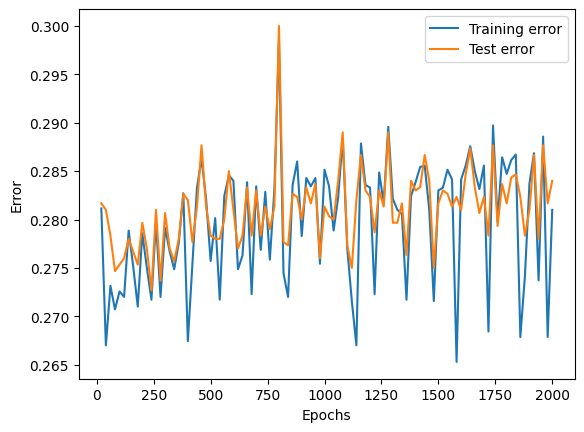
\includegraphics[width=0.6\columnwidth]{../plots/perceptron.png}
	\caption{Training and test errors of the perceptron varying the number of epochs}
	\label{fig:perceptron}
\end{figure}
\begin{figure}
	\centering
	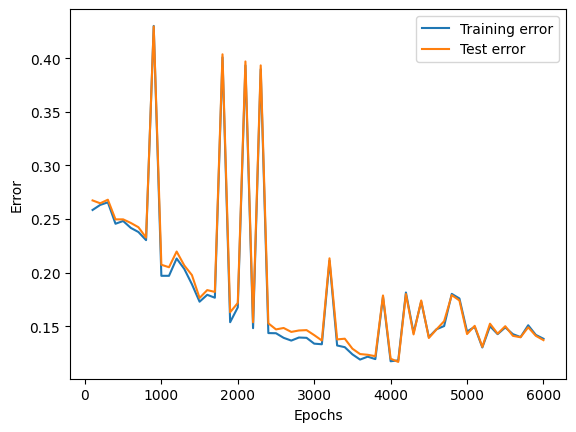
\includegraphics[width=0.6\columnwidth]{../plots/quad_perceptron.png}
	\caption{Training and test errors of the perceptron with quadratic feature extraction varying the number of epochs}
	\label{fig:quad_perceptron}
\end{figure}

\subsection{Kernel perceptron}
There may be room for improvement by applying a polynomial extraction of higher degree, but the training tends to be computationally intensive even for relatively small degrees and training sets, as the number of features explodes: considering 10 features, with a degree of 3, the number of expanded features would be 286, while with a degree set to 4 the number would be 1001. Kernel methods can be used to overcome this problem. 

\paragraph{Polynomial kernel}
Considering the polynomial kernel:
\begin{equation}
	K_d(x,x') = (1 + x^T x')^d
\end{equation}
figure \ref{subfig:kpoly_perceptron} shows errors using the kernel perceptron with different degrees $d\in \mathbb{N}$; the quality of predictions is far worse than the perceptron with quadratic feature expansion. Furthermore, predictors that used an odd degree performed visibly worse than the others. Also, higher degrees increase the gap between training and test errors, suggesting that large values lead the model to overfit. The kernel perceptron can be forced to make more than one scan on the dataset: instead of adding to a set $S$ the index of examples misclassified during the training, a counter of mistakes $\alpha_s$ is kept for each example $s$ and used as a multiplier. Thus, instead of computing the following function:
\begin{equation}
	h(x) = sgn\left(\sum_{s\in S} y_s K(x_s, x) \right)
\end{equation}
the prediction is evaluated through the following one:
\begin{equation}
	h(x) = sgn\left(\sum_{s=0}^{|S|} \alpha_s y_s K(x_s,x)\right)
\end{equation}

To find a good degree, values can be compared using cross validation: in particular, values between 2 and 10 are used, considering for now only one iteration of kernel perceptron to avoid long execution times. The best performing degree found for a single iteration of the polynomial kernel perceptron is 4, with a loss of 0.1427. To enhance prediction quality, the number of epochs is increased to 20, obtaining the errors shown in figure \ref{subfig:kpoly2_perceptron}; the values now approach the ones found in figure \ref{fig:quad_perceptron} for the perceptron with quadratic feature extraction.

\begin{figure}
	\centering
	\begin{subfigure}{0.45\columnwidth}
		\centering
		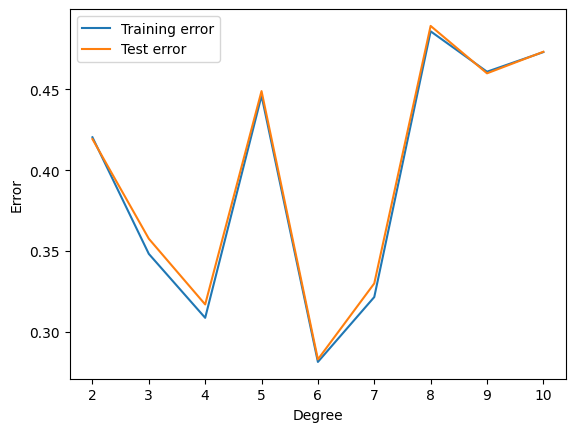
\includegraphics[width=\columnwidth]{../plots/kpoly_perceptron.png}
		\caption{}
		\label{subfig:kpoly_perceptron}
	\end{subfigure}
	\begin{subfigure}{0.45\columnwidth}
		\centering
		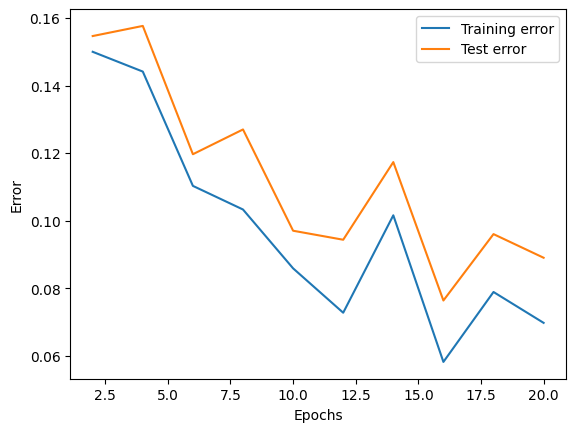
\includegraphics[width=\columnwidth]{../plots/kpoly2_perceptron.png}
		\caption{}
		\label{subfig:kpoly2_perceptron}
	\end{subfigure}
	\caption{Tuning phases of the perceptron with polynomial kernel. Figure (a) shows an initial search considering degrees from 2 to 10, figure (b) the plot with the error running more epochs on the best selected value using grid search with cross validation, that is $d=4$}
	\label{fig:kpoly_perceptron}
\end{figure}
\paragraph{Gaussian kernel}
To initially tune the $\gamma \in \mathbb{R}_{>0}$ hyperparameter of the Gaussian kernel:
\begin{equation}
	K_\gamma(x, x') = \exp\left(-\frac{1}{2\gamma} ||x-x'||^2\right)
\end{equation}
the values picked are in the interval $[10^{-3}, 10^2]$ in logarithmic scale, obtaining results shown in figure \ref{subfig:kgauss_perceptron}. The plot clearly shows how values lower than 1 cause overfitting, while values higher than 10 underfitting. 

The most promising range is explored performing cross validation considering 10 equidistant values of $\gamma$ in the interval $[0.5, 5]$. The best value observed during the search is $\gamma=1.5$ with a loss of 0.1245. A further improvement can be achieved by running the multiple epochs version of the kernel perceptron. The error obtained running up to 10 epochs of perceptron with Gaussian kernel and the selected value of $\gamma$ is shown in figure \ref{subfig:kgauss2_perceptron}.

\begin{figure}
	\centering
	\begin{subfigure}{0.45\columnwidth}
		\centering
		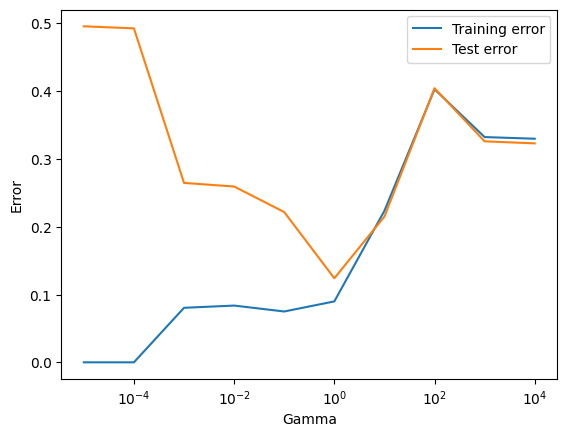
\includegraphics[width=\columnwidth]{../plots/kgauss_perceptron.png}
		\caption{}
		\label{subfig:kgauss_perceptron}
	\end{subfigure}
	\begin{subfigure}{0.45\columnwidth}
		\centering
		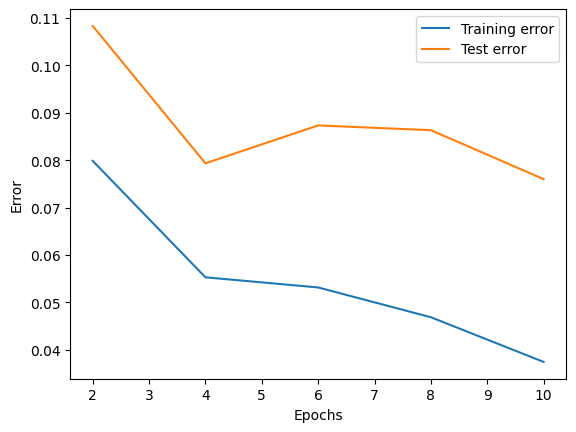
\includegraphics[width=\columnwidth]{../plots/kgauss2_perceptron.png}
		\caption{}
		\label{subfig:kgauss2_perceptron}
	\end{subfigure}
	\caption{Tuning phases of the perceptron with Gaussian kernel. Figure (a) shows an initial search considering a geometric sequence, figure (b) the plot with the error running more epochs on the best selected value using grid search with cross validation, that is $\gamma=1.5$}
	\label{fig:kgauss_perceptron}
\end{figure}

\section{Support vector machines}
Training SVM can be more challenging due to the presence of multiple hyperparameters to tune.
For this reason, grid search is performed on subsets of hyperparameters using cross validation for model evaluation. The number of folds in which the data is divided is 5. 
The dataset input for the validation is the one before preprocessing; a preprocessing step as described in section \ref{sec:preprocessing} is applied at every iteration of the cross validation, taking into account the division between training and test sets for the considered fold and always assuming that the content of the test set is unknown. 
In this section, grid search is applied twice: the first time it considers a large interval of values of the hyperparameters. In particular, the epochs considered for tuning are 1000, 5000, 10000, 15000 and the learning rate $\eta$ and regularization term $\lambda$ for the SVM objective function:
\begin{equation}
	f(w) = \frac{1}{m}\sum_{t=1}^m \ell_t(w) + \frac{\lambda}{2}||w||^2
\end{equation}
are from a geometric sequence of powers of $10$ in range $[10^{-3}, 10^2]$. 
The second run of grid search is used to explore the neighborhood of the promising values found in the first iteration.

Starting with SVM, the best loss value obtained through grid search in the first iteration is 0.2777, with 10000 epochs, $\eta=1$ and $\lambda=0.001$. 
For the second iteration, the considered numbers of epochs are 15000, 18000 and 20000, $\eta$ is selected from 10 equidistant values in the range [0.5, 5], while the considered interval for $\lambda$ is [0.0005, 0.005]. 
This time, the selected number of epochs is 20000, $\eta=0.5$ and $\lambda=0.003$, with an error of 0.2752. The errors during the training of an instance of SVM is shown in figure \ref{fig:svm}.
\begin{figure}
	\centering
	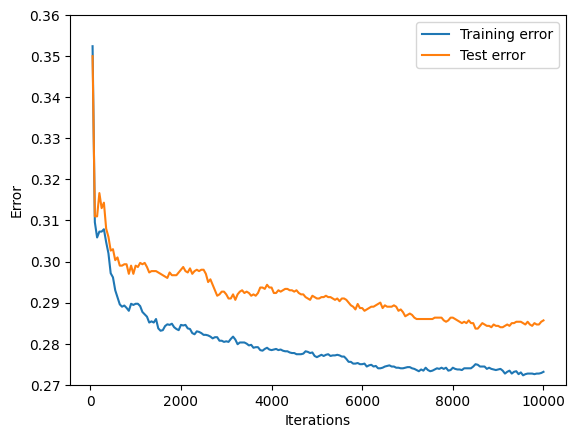
\includegraphics[width=0.6\columnwidth]{../plots/svm.png}
	\caption{Training and test errors on an instance of SVM with $\eta=0.5$ and $\lambda=0.003$}
	\label{fig:svm}
\end{figure}

\paragraph{Quadratic extraction}
As with the perceptron, the results can be improved by using polynomial feature expansion of degree 2. For parameter tuning, The grid search found in the first iteration 15000 as the number of iterations, $\eta=1$ and $\lambda=0.001$; the obtained loss is 0.0958. Continuing the exploration, the second run of grid search is performed with numbers of iterations equal to 15000, 18000 and 20000, for $\eta$, 10 equidistant values in range [0.3, 3] are considered and for $\lambda$, 10 equidistant values in the interval [0.0008, 0.008]. With this second search, a small improvement is found, with a loss of 0.0811; the selected number of iterations is 20000, $\eta=2.7$ and $\lambda=0.0008$. Looking at figure \ref{fig:quad_svm}, it can be seen that the curve of the errors tend to (almost) nullify its steepness after a much greater number of iterations with respect to the predictor on the non-expanded dataset.
\begin{figure}
	\centering
	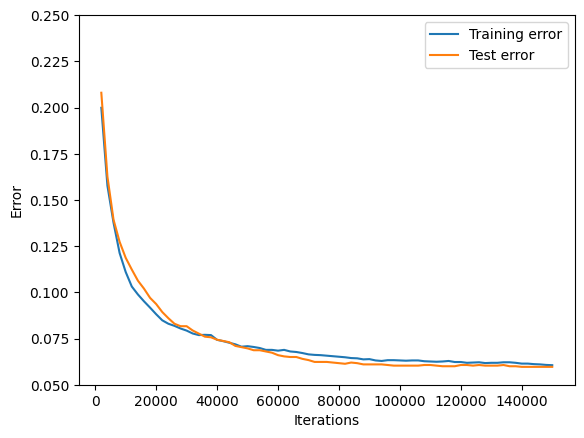
\includegraphics[width=0.6\columnwidth]{../plots/quad_svm.png}
	\caption{Training and test errors on an instance of SVM with quadratic feature extraction with  $\eta=2.7$ and $\lambda=0.0008$}
	\label{fig:quad_svm}
\end{figure}

\subsection{Regularized logistic classification}
The hinge loss $\ell_t$ can be replaced by the logistic loss in the objective function for SVM to obtain a regularized logistic classifier. The evaluation in the first run gave a loss of 0.2799 with 15000 iterations, 100 as $\eta$ and 0.001 as $\lambda$. After that, the neighborhood of the obtained hyperparameters is explored: the new grid search is performed using 15000, 18000 and 20000 as iteration counts, 10 equidistant values in the interval [20, 200] are used for $\eta$ and 10 equidistant values in the interval [0.0005, 0.005] for $\lambda$. the best value found this time is 0.2786 with 18000 iterations, $\eta=100$ and $\lambda=0.0005 $. The errors on an instance with the parameters just found, varying the number of iterations, is shown in figure \ref{fig:svm_log}. The predictor obtained with this version of Pegasos has a slightly higher error than the predictor with hinge loss. The surprising result is the use of a very high learning rate to reach a good quality of prediction.

\begin{figure}
	\centering
	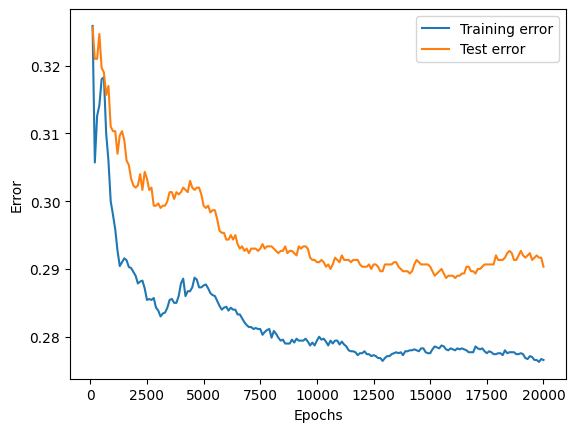
\includegraphics[width=0.6\columnwidth]{../plots/svm_log.png}
	\caption{Training and test errors on an instance of regularized logistic classifier with quadratic feature extraction with $\eta=100$ and $\lambda=0.0005$}
	\label{fig:svm_log}
\end{figure}
\paragraph{Quadratic extraction}
Applying grid search and cross validation with the usual parameters in the first iteration, the regularized logistic classifier with polynomial extraction of degree 2 gives 0.0976 as loss with 15000 iterations, $\eta=1$ and $\lambda=0.001$. Next, a grid search is performed with 15000, 18000, 20000 iterations, 10 equidistant values in the interval [0.3, 3] are used as $\eta$ and 10 equidistant values in the interval [0.0005, 0.005] as $\lambda$, obtaining a loss of 0.076 with $\eta=2.7$, $\lambda=0.0005$ and 20000 iterations. As in the case of SVM with hinge loss, quadratic extraction seems to require an higher number of iteration to stabilize around a certain value of error. The behavior of errors on a trained instance is shown in figure \ref{fig:quad_svm_log}.
\begin{figure}
	\centering
	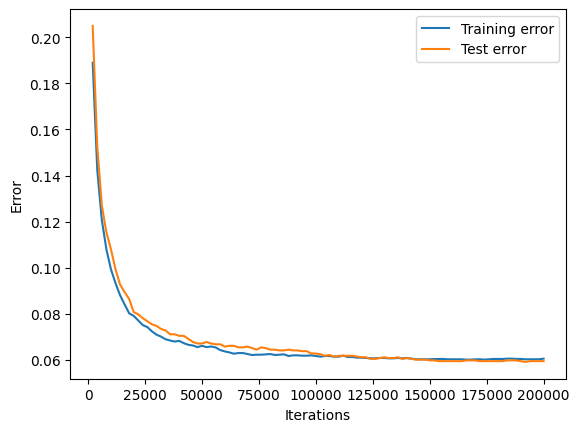
\includegraphics[width=0.6\columnwidth]{../plots/quad_svm_log.png}
	\caption{Training and test errors on an instance of regularized logistic classifier with quadratic feature extraction with $\eta=2.7$ and $\lambda=0.0005$}
	\label{fig:quad_svm_log}
\end{figure}

\subsection{Kernel SVM}

\paragraph{Polynomial kernel}
For the polynomial kernel version of Pegasos, the procedure of hyperparameters selection is quite similar to the one adopted until now. At first, a grid search is run considering degrees $d$ from 2 to 10, $\lambda$ values are picked from a geometric sequence of powers of $10$ in range $[10^{-3}, 10^2]$. The obtained loss considering 2000 iterations is 0.2013, $d=4$ and $\lambda=0.001$. For the second run, the grid search considers degrees between 3 and 5 and 5 equidistant $\lambda$ values between 0.0005 and 0.003. The resulting loss didn't change, the selected degree is still 4 and $\lambda=0.0005$. Figure \ref{fig:kpoly_svm.png} reports errors on an instance trained in 60000 iterations with the parameters obtained before. The errors through the iterations are overall descending, but there are visible spikes, suggesting that a high number of iterations are needed for reaching a more stable region. However, even training a model with 60000 iterations turned out to be costly in terms of time.

\begin{figure}
	\centering
	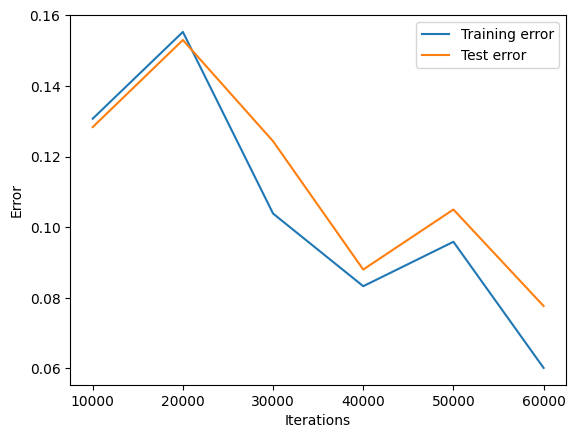
\includegraphics[width=0.6\columnwidth]{../plots/kpoly_svm.png}
	\caption{Training and test errors on an instance of SVM with polynomial kernel of degree 4 and $\lambda=0.0005$}
	\label{fig:kpoly_svm.png}
\end{figure}

\paragraph{Gaussian kernel}
For hyperparameters tuning of the Gaussian kernel version of Pegasos, a first run of grid search is performed by considering $\gamma$ and $\lambda$ values in a geometric sequence of powers of $10$ in the interval $[10^{-3}, 10^2]$. With 2000 iterations, the best parameters found are $\gamma=1$ and $\lambda=0.001$ and an error of 0.179. For the second run, the considered $\gamma$ values are 5 equidistant values in the interval $[0.4, 2]$, while for $\lambda$ they are 5 equidistant values in the interval $[0.0003, 0.0015]$. Performing 2000 iterations of Pegasos, the best loss obtained is 0.1723 with parameters $\gamma=0.8$ and $\lambda=0.0003$. An instance of SVM with Gaussian kernel using the parameters found with the second run of grid search, trained in 30000 iterations, is shown in figure \ref{fig:kgauss_svm.png}.

\begin{figure}
	\centering
	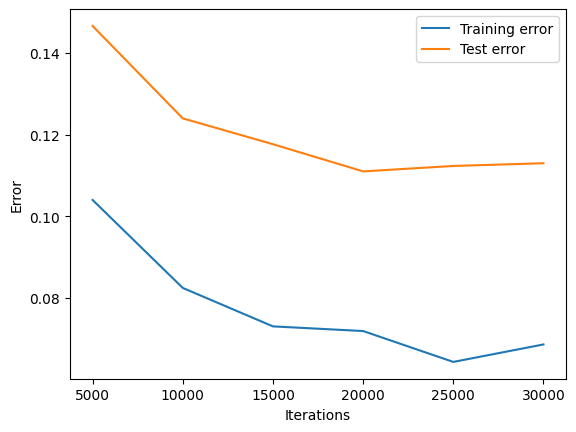
\includegraphics[width=0.6\columnwidth]{../plots/kgauss_svm.png}
	\caption{Training and test errors on an instance of SVM with Gaussian kernel with $\gamma=0.8$ and $\lambda=0.0003$}
	\label{fig:kgauss_svm.png}
\end{figure}

\section{Conclusions}
The dataset considered is almost certainly non-linearly separable, as the perceptron algorithm never converged during the experiments, while keeping an error quite stable around the same values through the epochs. Furthermore, the Pegasos algorithm failed to find the separating hyperplane too, even if it was capable of creating more reliable predictors than the perceptron, both optimizing the hinge loss and the logistic loss. A rationale for this result can be found in the way the hyperplanes are chosen by the two algorithms: an SVM explicitly optimize the objective function of the maximum margin separating hyperplane problem, giving a more robust predictor, instead of searching one of the available separating hyperplanes as in the case of perceptron. 

The use of quadratic extraction and kernel functions showed a huge improvement on the quality of predictions, with errors near to 0; in particular, the polynomial kernel with $d=4$ seemed to better describe the curve separating the two classes for the considered problem, both with the perceptron and SVM. The gaussian kernel seemed more prone to overfitting, with a larger gap between test and training errors, even with not too small values of $\gamma$. 

\paragraph{Computing times}
The kernelized versions of the considered algorithms turned out to be far more complex in terms of training and prediction times with respect to their basic versions. The comparisons\footnote{The times shown here and in the following are measured on a Ryzen 5 4500u with 8GB of RAM running Arch Linux with kernel 6.10.2-zen1-1-zen. The version of the Python interpreter is 3.12.4} between the perceptron, with and without quadratic extraction, and kernel perceptron is shown in figure \ref{fig:time_perceptron}, considering the best hyperparameters found in the previous sections.
The kernelized version shows the steepest curve for the training times measured on a training set of 7000 examples, but, most importantly, the basic perceptron prediction times (measured on 3000 examples) don't depend on the number of epochs run or on the training set size, as it's sufficient to compute the output from the vector weight whose size depends only on the number of features. The kernel perceptron, on the other hand, needs to keep a set of points that can grow unbounded and that needs to be scanned for each prediction.
A similar observation can be made for SVM, as it can be seen from figure \ref{fig:time_svm}; in this case a larger number of iterations can be performed with the same amount of time with respect to perceptron, as an iteration of Pegasos involve a random extraction and not an entire scan on the training set.
\begin{figure}
	\centering
	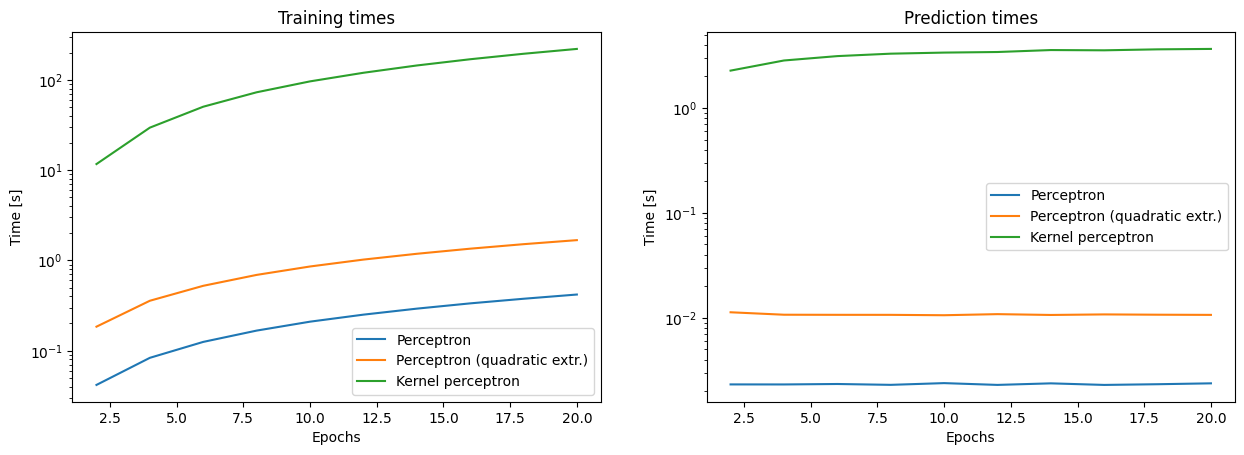
\includegraphics[width=\columnwidth]{../plots/time_perceptron.png}
	\caption{Training and prediction times comparisons between perceptron and kernel perceptron}
	\label{fig:time_perceptron}
\end{figure}
\begin{figure}
	\centering
	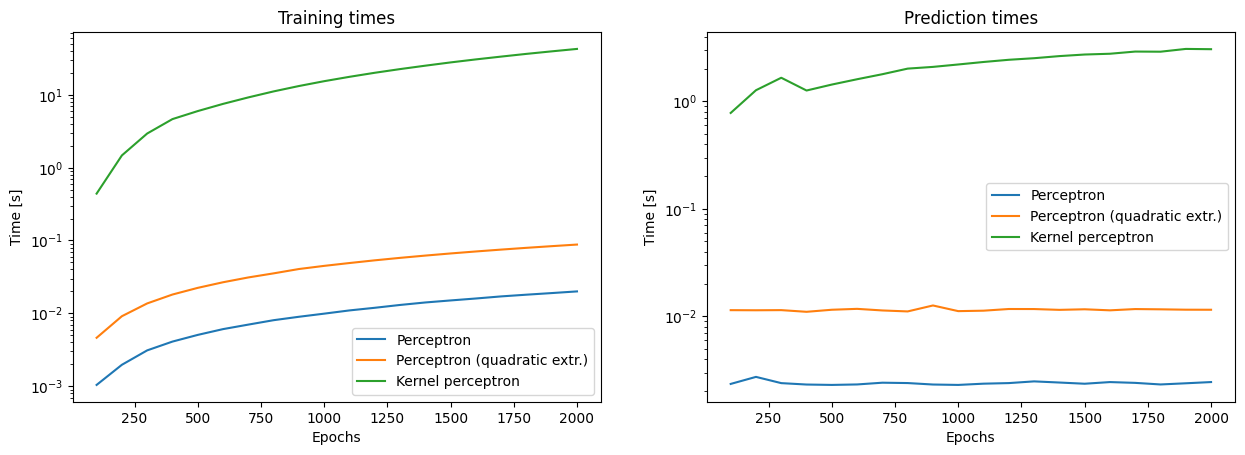
\includegraphics[width=\columnwidth]{../plots/time_svm.png}
	\caption{Training and prediction times comparisons between Pegasos and kernel Pegasos}
	\label{fig:time_svm}
\end{figure}
This shows that along with better predicting capabilities on non-linearly separable datasets, the kernelized algorithms come also with less scalability, which, in addition, prevented a better exploration of the hyperparameters spaces, the convergence of the stochastic gradient descent towards the minimum of the SVM objective function or to find a separating curve (in case there is) if considering the perceptron, all in reasonable amounts of time. Looking at the results, polynomial feature expansion can be a better choice when the number of features is relatively low and so is the degree $d$, as in the case with $d=2$.

\end{document}